\chapter{Implementation}
\label{chapter-implementation}

As a part of this thesis, we designed a simple tool able to work with our dataset and execute various tasks over it. The main idea was to unify the interface for models, so many different models can be run just via command line. This proved to be essential when running many models concurrently in Metacentrum or in the local machine. 

The whole tool is written in Python 3.6 and it is accessible via one command-line interface.

\section{Used technologies}

\subsection{Pandas}

To work with CSV files of a length of more than 30 million lines, one does need to use the appropriate framework for it. We chose the pandas\cite{pandas} library. Actively supported today by a community, it is a BSD-licensed library providing high-performance, low-level optimized and easy-to-use data structures for data analysis for \textit{Python} programming language. Pandas stores its data in so-called dataframes\cite{pandas-df}, which are working on the same principle as in the \textit{R} language. They can store two-dimensional size-mutable heterogeneous tabular data and allow arithmetic operations align on both row and column. Furthermore, pandas can work with with huge CSV files using python generators.

\subsection{TensorFlow}

TensorFlow\cite{tensorflow} is an open source software library for high performance numerical computation. Tensorflow was developed by the Google Brain team for internal Google use. It was released under the Apache 2.0 open source license on November 9, 2015 Its flexible architecture allows easy deployment of computation across a variety of platforms (CPUs, GPUs, TPUs), and from desktops to clusters of servers to mobile and edge devices. Originally developed by researchers and engineers from the Google Brain team within Google’s AI organization, it comes with strong support for machine learning and deep learning and the flexible numerical computation core is used across many other scientific domains. Its core is written in C++ and CUDA, thus it is highly optimized for parallel computations on GPU.

\subsection{Keras}

Keras\cite{keras} is arguably one of the most popular python tensorflow frontends for a quick and simple definition of networks. In comparison to tensorflow, Keras is very layer-oriented and has an intuitive user friendly API. All models, that we trained were defined over Keras framework. The simplicity of Keras framework can be shown in an example of a concrete model, that we used. The whole model is defined in just 5 lines of code:

\begin{minted}[ framesep=2mm,
                autogobble,
                frame=lines]{python}
import keras
inputs = keras.layers.Input(shape=(input_dimension,))
x = keras.layers.Dense(1024, activation='relu')(inputs)
outputs = keras.layers.Dense(output_dimension, activation='softmax')(x)
model = keras.models.Model(inputs=inputs, outputs=outputs)
model.compile(loss=keras.losses.categorical_crossentropy,
              optimizer=keras.optimizers.Adadelta(),
              metrics=['acc'])

\end{minted}

\subsection{Scikit-learn}
 
Before trying any neural network models, we tried to use simple models first. We chose the sklearn\cite{scikit} package, the native package for basic machine learning and evaluation. We used classifiers such as KNN, Naive Bayes, decision trees or support vector classifiers\footnote{List of all possible classifiers can be found in \url{http://scikit-learn.org/stable/supervised\_learning.html\#supervised-learning}}. 

\subsection{Docker}

\label{docker}

Initially, the tool was developed on the local Linux machine, because it was dependent on third-party Unix binaries, as well as it was later deployed to Metacentrum cloud, which is Unix native. However, we needed to develop and run it also on other architectures. One approach is to install virtual machines on the desired host, setup Unix environment and then run the tool. The better, more modern approach would be to use containers, namely Docker\cite{docker}.

Docker encapsulates the application, running environment, dependencies and architecture into a self-contained unit that can run anywhere. It is a more lightweight virtual machine because containers in comparison to virtual machines share the host system's kernel with other containers\cite{docker-blog}. By defining dockerfile, we provided any user the option to run this tool on its own local host.

\subsection{Python generators}

\label{python-generators}

During the training process, we were working with huge files with over a couple of millions of lines. Even as raw strings, that could take up to 2 GB of memory. Furthermore, we transformed the keys into numpy arrays, which was infeasible memory-wise as it could take easily more than 20-25 GB of RAM. Rather than allocating such memory in Metacentrum, one can provide a better solution - python generators\cite{python-gen}. 

Generator functions allow you to declare a function that behaves like an iterator, i.e. it can be used in a for loop. The main advantage is that the data is fetched during the runtime as the iteration of the for loop is always called on demand.

\begin{minted}[ framesep=2mm,
                autogobble,
                frame=lines]{python}
def get_data():
	n = 1
	while True:
		yield n
		n += 1
		
for n in generate_numbers():
	...
\end{minted}

This simple example shows how to generate natural numbers. Instead of natural numbers we simply take a chunk of lines from the source CSV file resulting in saving the memory consumption. Therefore we can run huge datasets also in local machine as well as take smaller resources on Metacentrum, thus increasing our chance of running our job in the 

\subsection{Click}

As our tool provides only command line interface, we chose the Click package\cite{click}, a command line interface creation kit. It provides decorator options for defining arguments and options with validation and automatic help generation. As a framework, it suited the necessary needs for the application and sped up the development process.

\section{Tasks}

During the implementation process, several distinct tasks were implemented in order to work with the original dataset, prepare the data for models to train and then classify. Figure \ref{figure-model} shows the flow of the application and its data. We named these tasks \textbf{SCAN, ANALYZE, GENERATE, TRAIN} and \textbf{CLASSIFY}.

We obtained a dataset in the form of around 2000 CSV files. First of all, we wanted to automate extracting the keys from distinct files and set up class labels to it. Therefore, \textbf{SCAN} task was implemented. We used it mainly to transform given dataset, which was difficult to extract keys from into more compact one. The transformed dataset could be used more efficiently for analysis and generating new ones.

The newly generated compact dataset was then subjected to full analysis of features. For this purpose \textbf{ANALYZE} task was implemented. We used it to generate the relative frequency of features, that we presented in the chapter \label{chapter-analysis}.

Another task \textbf{GENERATE} was used to prepare custom generated datasets for machine learning models. Its main purpose was to be able to generate datasets with different class labels, replicate keys in training dataset, skip group, skip files, merge several groups into one and others. We used this task throughout the whole training process to create datasets for models and tune them if the model was struggling in training.

The main task \textbf{TRAIN} was applied to the custom generated datasets. Its main purpose was to be able to feed data into the model, monitor performance and report the results of the training. Models are sharing the same interface. This allows to implement new model relatively simply and use the whole task for any model.

Models that are performing well can be used, evaluated and tested via \textbf{CLASSIFY} task using the same shared core with \textbf{TRAIN}.

\begin{figure}[H]
\centering
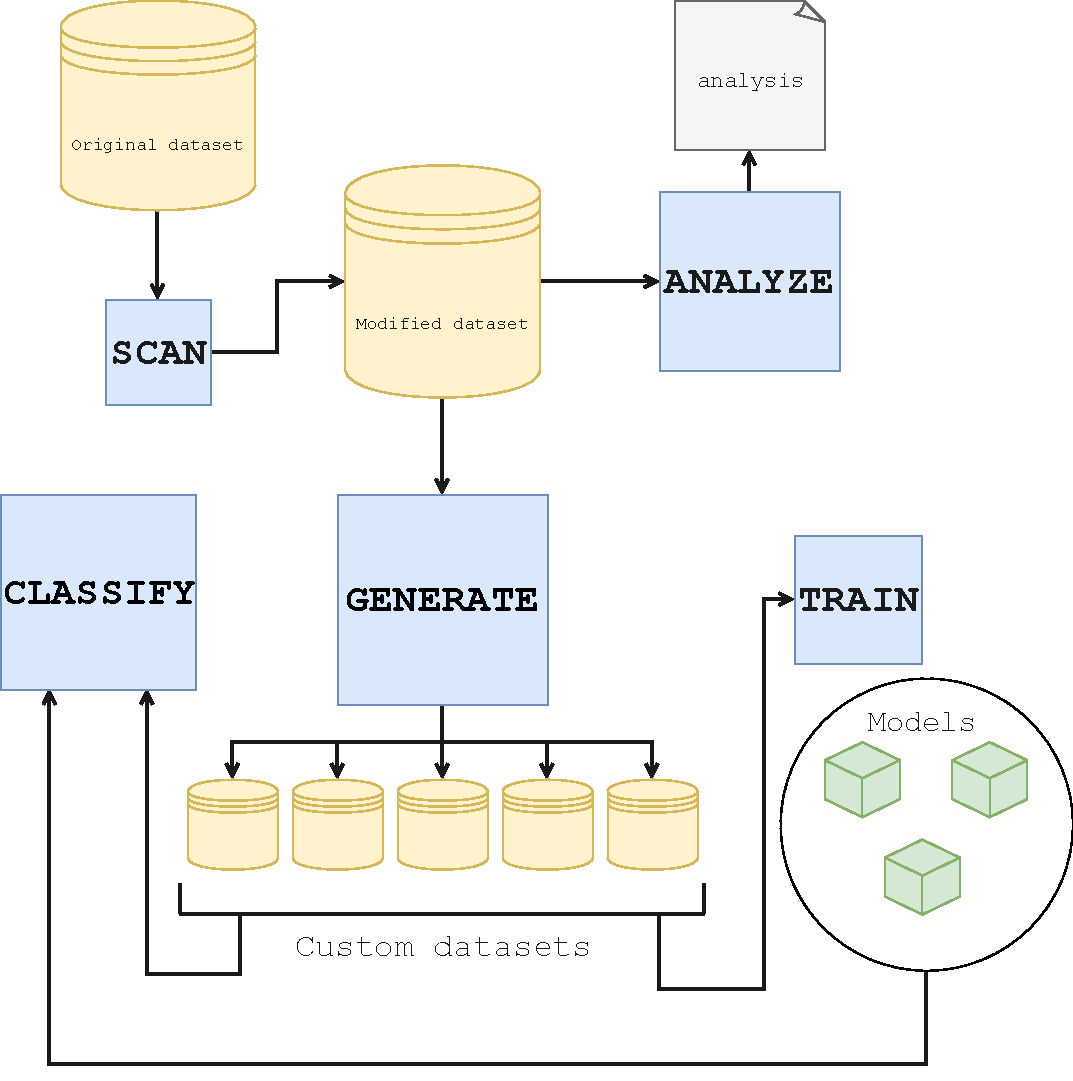
\includegraphics[width=0.65\textwidth]{tex/images/thesis_model}
\caption{Diagram of the application flow shows 5 distinct tasks (SCAN, ANALYZE, GENERATE, TRAIN, CLASSIFY) that we used to work with our dataset and perform machine learning on them.}
\label{figure-model}
\end{figure}

\subsection{SCAN task}

The original dataset was in the form of a directory hierarchy, where there was no specific namespace for different key length and sources. We needed a task to be able to create groups of sources, that would be corresponding to the same label. The using this grouping generate a new dataset, which is wel; structured and easier to analyze.

\textit{SCAN} task is using simple string matching with required (positive) keywords and forbidden (negative) keywords. Then it iteratively loops through all CSV files in given root directory and looks for CSV files that contain any positive keyword and not containing any negative keyword. Keywords are passed to the task via JSON structure. In Here is an example of a JSON filter we defined over the original dataset, which scan all sources from group 13 with bitlength of 1024: 

\begin{minted}[ framesep=2mm,
                autogobble,
                frame=lines]{json}
{
    ...
    "13": {
        "required": [
            "Botan_1-5-6",
            "Botan_1-11-29",
            ...
            "WolfSSL_3-9-0",
            "WolfSSL_3-10-2"
        ],
        "forbidden": [
            "PGP_SDK_4_FIPS",
            "Libgcrypt_1-7-6_FIPS",
            "512",
            "2048"
        ]
    }
}

\end{minted}

\noindent
As a result, we obtain a JSON file, which contains groups of sources with given label and a list of individual sources with the number of keys in them. This JSON file is used further by \textit{GENERATE} task. Below we show the example of a generated JSON file from the previous filter:

\begin{minted}[ framesep=2mm,
                autogobble,
                frame=lines]{json}
{
    ...
     "13": {
            "group_name": "13",
            "keys_total": 31911043,
            "sources": [
                {
                    "length": 50001,
                    "name": "Feitian JavaCOS A22",
                    "path": "/Card/Feitian JavaCOS A22 1024b/UnknownICSN 1.csv",
                    "read_lines": 0
                },
                ...
            ]
     }
}

\end{minted}

\subsection{ANALYZE task}

The problem with working with huge CSV files is memory consumption, as we usually are not able to load all keys into RAM at once. Fortunately, pandas\cite{pandas} library offers reading and processing such files in chunks of lines. 

When analyzing a huge file, we iterate it in chunks, extracting values for features from every key and then just incrementing the corresponding counter. In the end, we print the analysis to the user.

\begin{figure}[h]

\centering
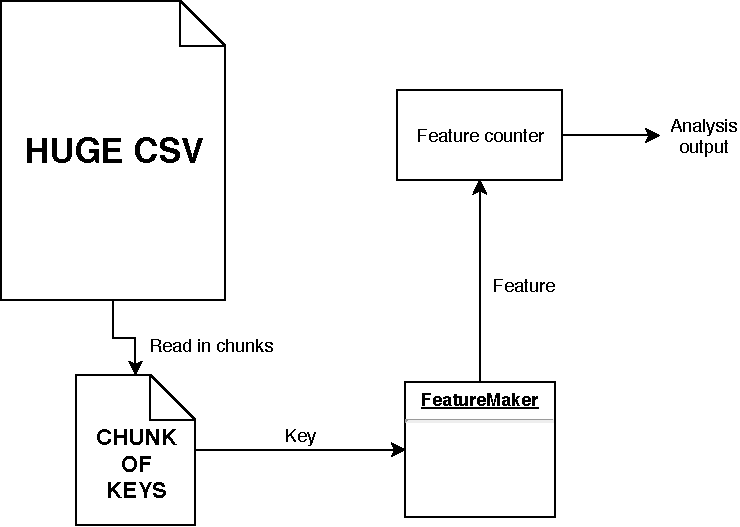
\includegraphics[width=0.5\textwidth]{tex/images/analyze_task}
\caption{\textit{ANALYZE} task flow.}

\end{figure}

Using \textit{SCAN} and \textit{GENERATE} we transformed the dataset to fit our purposes. We extracted all keys from each of available 64 sources of different key lengths and merged them all into single CSV files\footnote{i.e. for source 01 with we obtained 3 files, each with 512/1024/2048 keys respectively}. 

Having the dataset decoupled into several smaller CSV files, we could actually perform an analysis on each of these files distributively in the CESNET cloud.

\subsection*{Feature Maker}

\label{feature-maker}

When analyzing the dataset, we obtained features to use in machine learning. Having them hardcoded would not be the best approach, as new features may occur or some features may not be used for some specific model. 

That is why we designed the Feature Maker. It is essentially a class, that is dedicated to the transformation of a raw key into the specific feature vector. Features may be added during runtime dynamically, usually via a configuration file. It gives us freedom of choosing a different set of features with every model (or during the analysis as well). Also, adding new feature does not change any other code, but the Feature Maker class itself. The features implemented so far:

\begin{itemize}

\item \textit{modulo} - can return either binary vector class (useful for machine learning) or remainder as a decimal number (useful for analysis)
\item \textit{bit} - returns specific bit (useful for mask in machine learning and analysis)
\item \textit{line} - returns whole line (shortcut of taking every bit)
\item \textit{xor} - return xor of two specified bits

\end{itemize}

\noindent
Using this class is a question of couple lines of code. In the following simplified example, we define the feature maker, assigned three features to it (modulo 3, modulo 7 and 38-th LSB), then call the \texttt{get\_features\_from\_keys} which extract features for us. Adding or removing features can be performed between 2nd and 4th line of code:

\begin{minted}[ framesep=2mm,
                autogobble,
                frame=lines]{python}

fm = FeatureMaker()
fm.add('mod3')
fm.add('mod', {'n': 7})
fm.add('bit', {'i': 37})
features = fm.get_features_from_keys(keys)

\end{minted}

\subsection{GENERATE task}

One of the most important tasks we had to implement was \textit{GENERATE} task. Given our modified dataset, we needed to generate smaller samples on which we could train different models. The whole process is managed by a Generator object, which reads the data specified by sources in a JSON file provided from \textit{SCAN} task. It is responsible for preparing the datasets for \textit{TRAIN} task. The Generator provides functionality to:

\begin{itemize}

\item generate single large CSV file
\item generate triplet of CSV files (train / test / valid) with ratio provided by the user
\item shuffle target CSV file
\item relabel individual groups and merge several groups together 
\item skip any source or the whole group of sources
\item take an arbitrary number of keys per group
\item take an arbitrary number of keys per line (meaning taking several keys as one line in target CSV file)
\item multiply keys in training data (useful for sampling, when a group has a limited amount of keys)

\end{itemize}

The advantage of such an approach is that using the same original dataset, the user can generate a number of different datasets with his custom labels just by changing the configuration. Given the user's settings, the Generator works in a couple of steps:

\begin{enumerate}

\item prepare the temporary CSV file that will store the new lines

\item prepare new labels mapping (user can merge different sources together, some labels might be unused)

\item iterate through sources specified in JSON

\item skip sources or groups that user specified

\item prepare a random sample of lines that will be read from the source, then read these lines in batches

\item prepare the line for the big CSV file (user can take more keys as one line in the final CSV)

\item multiply training sample by the ratio specified by the user

\item append line to the temporary file

\item shuffle temporary file and return as a new file (the final dataset)

\end{enumerate}

\noindent
All user's settings are specified in section \ref{cli}.

\subsection{TRAIN task}

The main task defined was task \textit{TRAIN}. As we provided all the tasks to prepare our datasets, we needed to implement the process of training the classifiers. The main idea was to split the process into two main logical units. The responsibility of the first one is to load the datasets a pass them on to the models. The second unit is models themselves.

\subsection*{Loader}

The \texttt{Loader} interface is a part of the core of the application. It provides two main function to feed data to the models:

\begin{itemize}

\item \texttt{get\_data()} - loads the whole file into memory and returns the numpy arrays, that can be fetched into the model (was necessary when working with models from scikit learn, that could not work with python generators). This is not suitable for larger files as they often don't fit into memory at once.

\item \texttt{get\_data\_generator()} - as mentioned in subsection \ref{python-generators}, when working with large files, it is more desirable to read them in chunks. Keras models do support training using python generators if we do provide one.

Reading the CSV in chunks using pandas, we extracted the features in every generator iteration and then yielded the data for the neural networks.

\end{itemize}

\noindent
As we were using two types of classifiers (from \textit{sklearn} and \textit{keras} libraries) and two types of datasets from \textit{GENERATE} task (either one big CSV file, or the CSV triplet), we provided two classes, that implemented this common interface:

\begin{itemize}

\item \texttt{LoaderSingle} - receive only one CSV file, and the split set ratios of the dataset. It computes the random permutation on lines, which are then distributed into their train / valid / test sets respectively. It directly corresponds to the single CSV files generated from \textit{GENERATE} task and it was implemented first.

\item \texttt{LoaderDataset} - the later implementation, receives the CSV triplet (train / test / valid) and does not need to compute the random permutation (which is memory consuming by itself). It directly corresponds to the CSV triplet from \textit{GENERATE} task.

\end{itemize}

\noindent
The feature extraction from individual keys was done by \texttt{FeatureMaker} class with features specified by the user. More details were mentioned in the subsection \ref{feature-maker}

\subsection*{Models}

When designing the models, the main focus was put on extensibility. We implemented a common \texttt{Model} as a plain abstract class using the python \textit{abc} module\footnote{\url{https://docs.python.org/3/library/abc.html}}. This allowed us to implement many models while keeping the same interface. Furthermore, as it is expected, that this application will be used later in the research, it is simple to add any another model just by implementing this interface and its methods:

\begin{itemize}

\item \texttt{fit()} and \texttt{fit\_generator()} - the model is given training and validation data in the form of either numpy arrays (\texttt{fit}) or an iterator (\texttt{fit\_generator}). The model trains itself.

\item \texttt{predict()} - given the input numpy vector, the model returns the prediction

\item \texttt{score()} - given the test data, the model returns an evaluation of itself

\item \texttt{get\_model\_info()} - return description as a string (used for logging the output)

\item \texttt{save()} - save model to given directory path

\item \texttt{load()} - load model from given directory path

\end{itemize} 

We implemented an interface to work with models from \texttt{scikit} library and multilayer perceptrons from \texttt{keras} library. For both of them, we implemented interfaces, that were direct children of the common \texttt{Model} interface. They implemented all the necessary interface methods to adapt them to used libraries. All the used models then inherited from this interface. The hierarchy can be seen in figure \ref{model-inheritance}.

\begin{figure}[H]

\centering
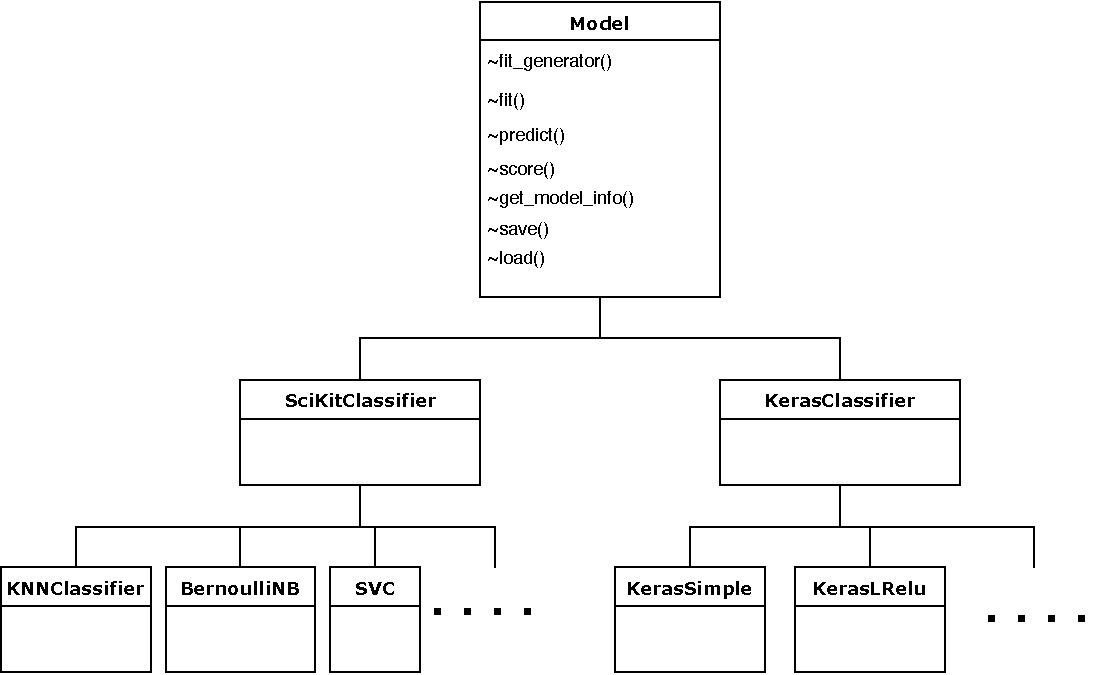
\includegraphics[width=0.75\textwidth]{tex/images/model_inheritance}
\caption{The hierarchy of implementation of the common \texttt{Model} interface. The second level groups the common logic for given library, the bottom level are individual implementations.}
\label{model-inheritance}

\end{figure}

From \texttt{scikit} we implemented most of the models listed in the documentation\footnote{\url{http://scikit-learn.org/stable/supervised\_learning.html\#supervised-learning}} (i. e. \texttt{KNN, NB, DecisionTree, SVC} and others). From \texttt{keras}, we implemented different multilayer perceptrons with topology specified by the user. Topology specifies hidden layers with their activation and the number of neurons, loss function, metrics, optimizer and activation of the output layer as JSON (example below).

\label{models-json}
\begin{minted}[ framesep=2mm,
                autogobble,
                frame=lines]{json}

 "Keras10": {"base": "KerasSimpleClassifier",
             "name": "Keras Multilayer Perceptron",
             "topology": {"hidden_layers": [{"activation": "relu",
                                             "number_of_neurons": 4096}],
                          "loss": "categorical_crossentropy",
                          "metrics": ["acc"],
                          "optimizer": "Adadelta",
             "output_layer": {"activation": "softmax"}}},

\end{minted}

\noindent
The models are trained in epochs, and after the training ends, they are evaluated with metrics defined in subsection \ref{nn-metrics}.

\subsection{CLASSIFY task}

The last (and for the end user, the most important one) is the \textit{CLASSIFY} task. The user compares trained models to target CSV file and can either evaluate the model based on the labels given in the CSV file (similarly as in \textit{TRAIN} task) or can generate new labels for his dataset (useful for tagging unknown data).

\section{Command line interface}
\label{cli}

We designed a simple CLI application using click library. The user can configure the application with the arguments or YAML configuration file (by default \textit{settings.yml}). Command line arguments have priority over YAML settings. For every task, the user can print help with description of the task, example of usage, arguments and yaml settings. The complete documentation with examples can be found in appendix \ref{appendix-running}.

\section{Multi platform development}

As we are using the third party binary, that is necessary for shuffling the datasets in \textit{GENERATE} task, the application needs to run in Linux Debian.

We were developing the application on Debian and Mac OS X. To be able to run it in Mac OS X we had to use the Docker container specified in the section \ref{docker}.

For this purpose we provided our code with simple dockerfile, that can run the application in its native environment on any platform:

\begin{minted}[ framesep=2mm,
                autogobble,
                frame=lines]{docker}

FROM python:3.6-slim
RUN mkdir -p /opt/rsa-ml
WORKDIR /opt/rsa-ml
COPY requirements.txt .
RUN pip install --no-cache-dir -r requirements.txt
COPY . .

\end{minted}

\noindent
Example of usage can be found in appendix \ref{appendix-docker}.

\section{Metacentrum}

The final step of the implementation process was to run the code in the cloud. We used batch jobs\cite{metacentrum} that run in the CESNET cloud - Metacentrum. One can simply run these scripts with more powerful resources that his local machine. We used it, in particular, to try many models in parallel, usually running for a couple of days. Batch jobs were run via a shell script. Example can be found in appendix \ref{appendix-metacentrum}.
